
\subsection{Test cases}
The (LE) variant was worth a test from my point of view (before I alternatively start with the Taylor variant, if necessary), because it as relatively easy to implement and storing the additionally needed interface values from the time step $t_{n-2}$ does not require much space. 
\newpage
\subsubsection{Case 1}
Let's start with a very simple test with only one obstruction which is completely contained in one mesh. Please note the displayed ranges.
\begin{figure}[H]
\begin{center}
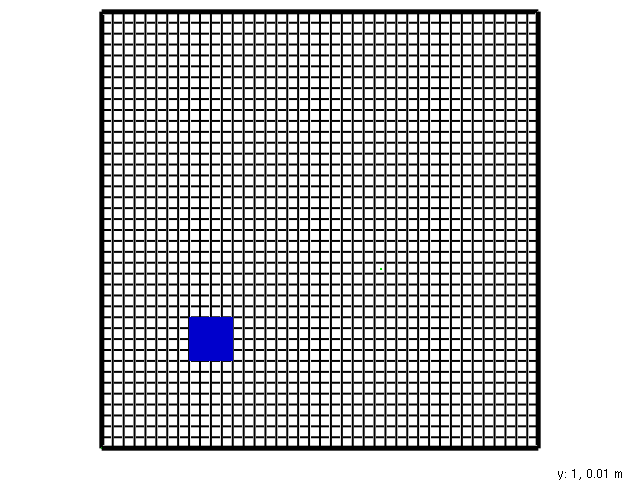
\includegraphics[width=3.5cm]{\figPath/a1_s0001.png}
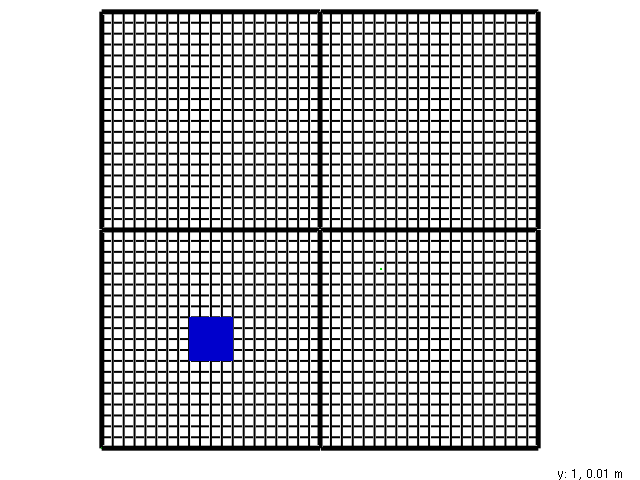
\includegraphics[width=3.5cm]{\figPath/a4_expol_s0000.png}
\end{center}
\caption{Case 1}
\label{FIG_MGM_Grid}
\end{figure}

Then the simple setting (SM) gives

\begin{figure}[H]
\begin{center}
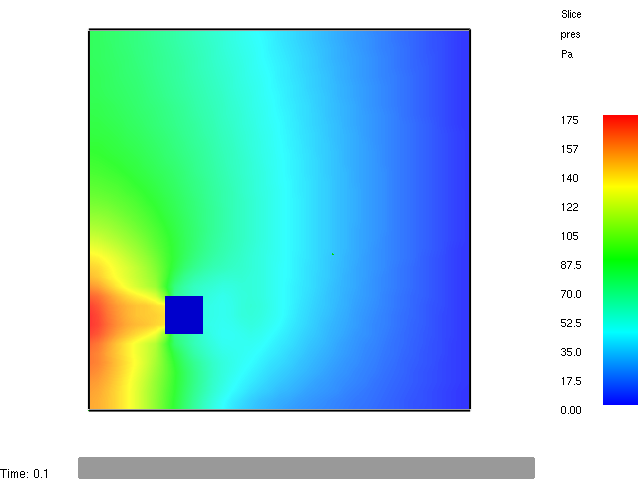
\includegraphics[width=7cm]{\figPath/a1_0062.png}
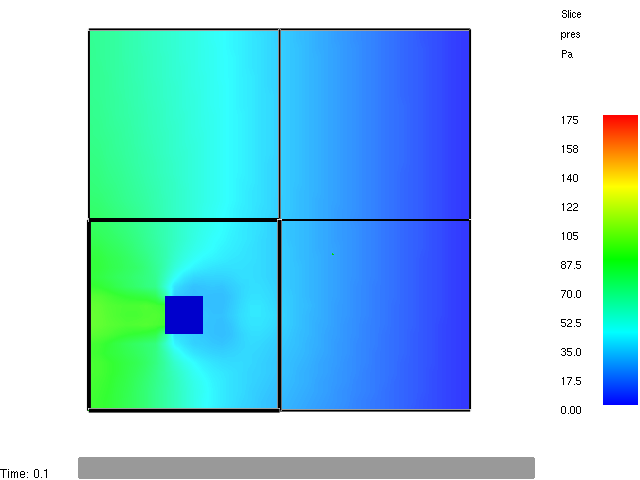
\includegraphics[width=7cm]{\figPath/a4_simple_0062.png}
\end{center}
\caption{Simple setting (SM) for Case 1}
\label{FIG_MGM_Grid}
\end{figure}


and the linear extrapolation setting (LE) gives

\begin{figure}[H]
\begin{center}
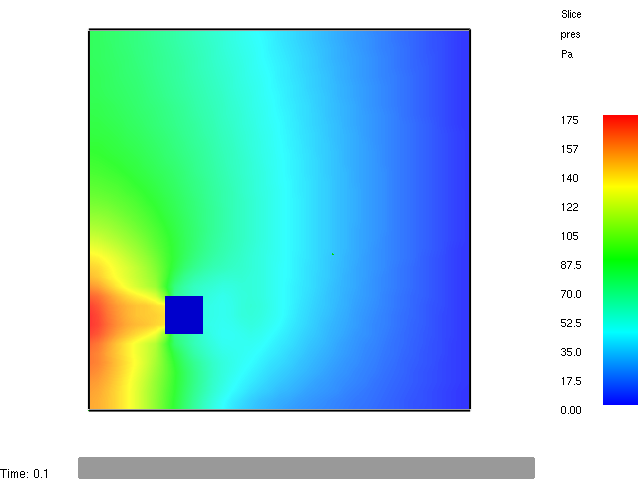
\includegraphics[width=7cm]{\figPath/a1_0062.png}
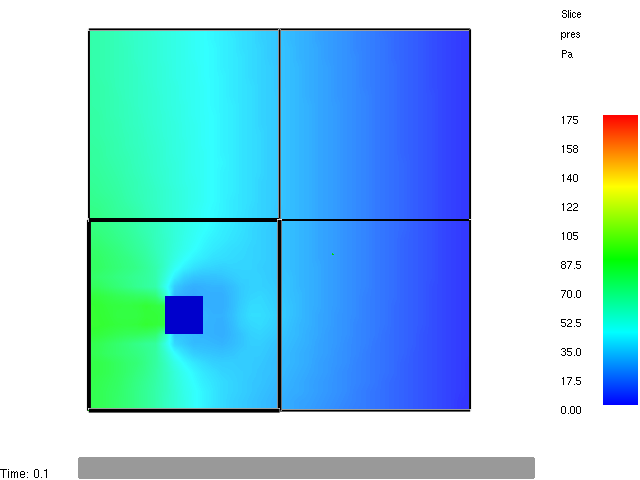
\includegraphics[width=7cm]{\figPath/a4_expol_0062.png}
\end{center}
\caption{Linear extrapolation setting (LE) for Case 1}
\label{FIG_MGM_Grid}
\end{figure}


\subsubsection{Case 2}
Let's start with a very simple test with only one obstruction which is completely contained in one mesh. Please note the displayed ranges.
\begin{figure}[H]
\begin{center}
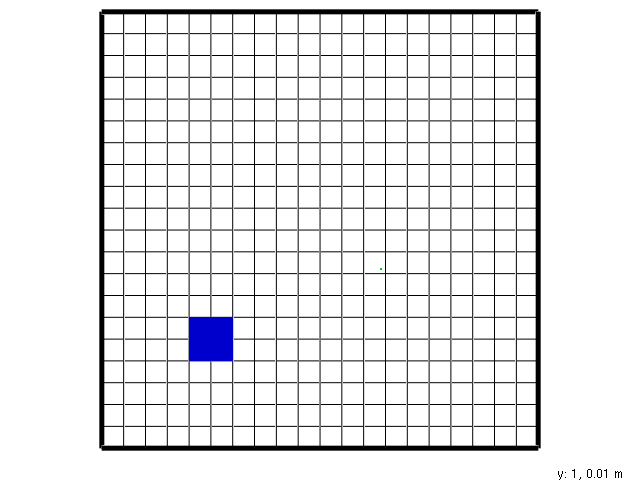
\includegraphics[width=3.5cm]{\figPath/mgm1_grid.png}
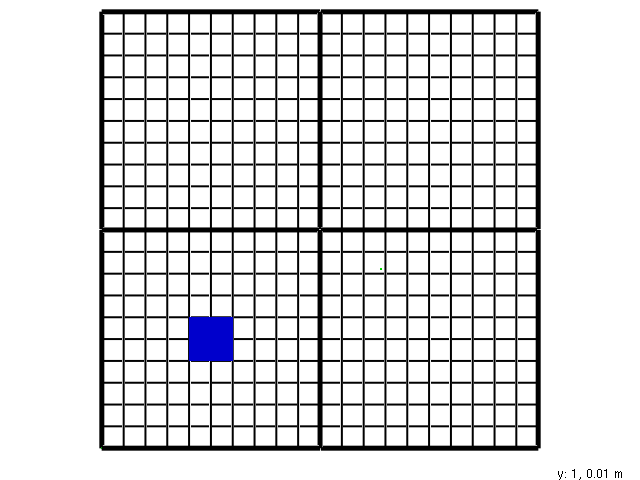
\includegraphics[width=3.5cm]{\figPath/mgm4_grid.png}
\end{center}
\caption{Case 2}
\label{FIG_MGM_Grid}
\end{figure}

Then the simple setting (SM) gives

\begin{figure}[H]
\begin{center}
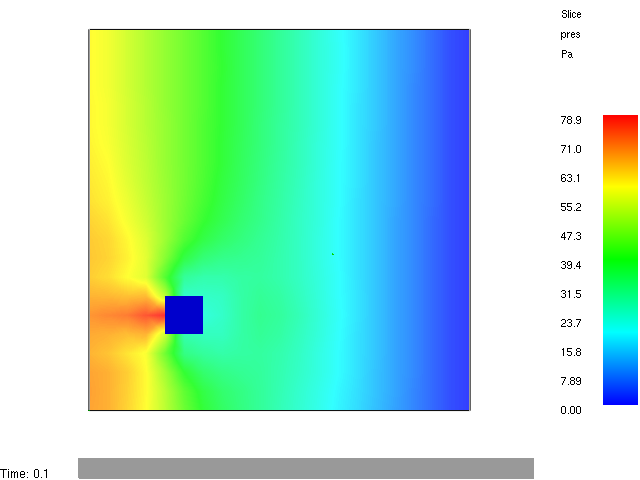
\includegraphics[width=7cm]{\figPath/mgm1.png}
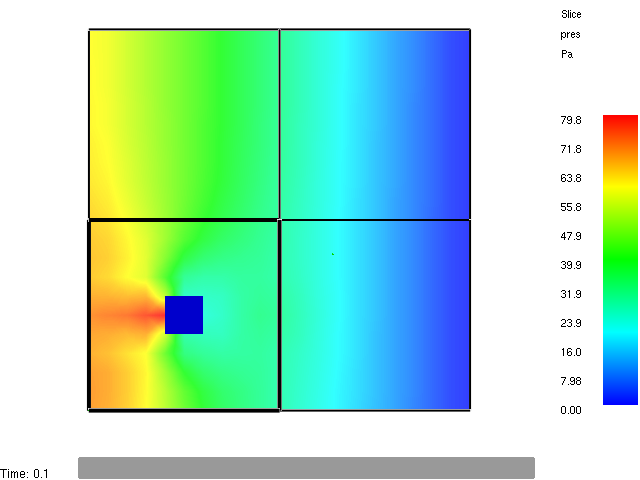
\includegraphics[width=7cm]{\figPath/mgm4_simple.png}
\end{center}
\caption{Simple setting (SM) for Case 2}
\label{FIG_MGM_Grid}
\end{figure}


and the linear extrapolation setting (LE) gives

\begin{figure}[H]
\begin{center}
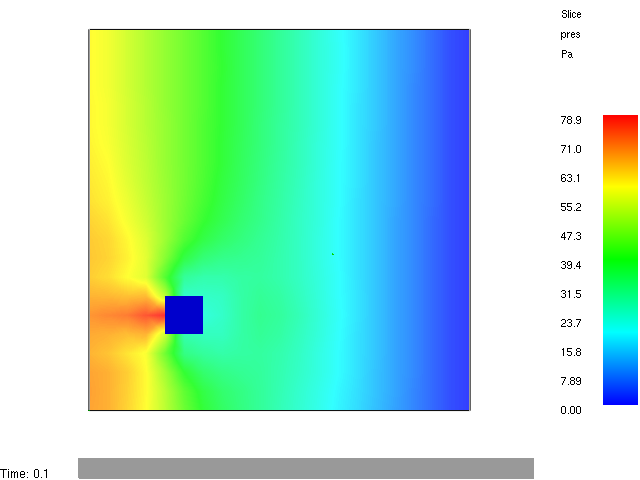
\includegraphics[width=7cm]{\figPath/mgm1.png}
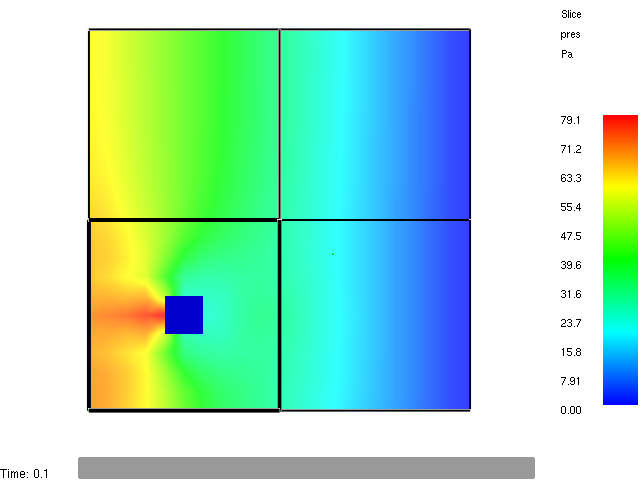
\includegraphics[width=7cm]{\figPath/mgm4_expol.png}
\end{center}
\caption{Linear extrapolation setting (LE) for Case 2}
\label{FIG_MGM_Grid}
\end{figure}




